\documentclass[t]{beamer}

\mode<presentation>
{
  \usetheme[german]{KIT}
  \setbeamercovered{transparent}
  \setbeamertemplate{enumerate items}[ball]
}

% \usepackage{epstopdf}
% \usepackage{pgf}
% \usepackage{tikz}
% \usepackage{pgflibraryshapes}
% \usepackage{ifthen}
% \usepackage{listings}
% \usepackage{xcolor}
% \usepackage{pslatex}
\usepackage{german}
\usepackage{graphicx}
\usepackage{booktabs}
\usepackage{textcomp}
\usepackage{tikz}
\usepackage{marvosym}
\usetikzlibrary{arrows,%
                petri,%
                topaths,%
                automata}%
\usepackage{tkz-berge}
\usepackage{xcolor,colortbl}

\usepackage{amsmath, amssymb, wasysym}
% \usepackage{tikz}
\usetikzlibrary{arrows,shapes,decorations.pathreplacing,calc,shadows}
\usepackage{calc}
\usepackage{ifthen}
\usepackage{url}
% \usepackage{pgfarrows}
% \usepackage{soul}
% \usepackage{comment}
% \IfFileExists{luximono.sty}{\usepackage[scaled]{luximono}}{}
% \usepackage{colortbl}
% \usepackage{booktabs}
% \usepackage{array}
% \usepackage{keylogo}
\usepackage[utf8]{inputenc}
\usepackage[T1]{fontenc}

% \newboolean{tutors}
% \setboolean{tutors}{false}
%%%%%%%%%%%%% LSTLISTING %%%%%%%%%%%%%%%%%%%%%%%%%%%%%%%%%%%%%%%%

% \lstdefinelanguage{VCC}[]{C}
% {
%   morekeywords={assert, assume, invariant, true, false, requires, ensures,
% writes},
%   moredelim=[is][\alert]{/+}{+/},
%   moredelim=[is][\color{gray}]{/-}{-/}
% }
% 
% \lstdefinelanguage{CASL}[]{}
% {
%   keywords={spec, then, end, ops, op, preds, forall, else, free, type, when,
%   within, implementation}
% }
% 
% \lstdefinelanguage{JML}[]{Java}
% {
%   moredelim=[is][\alert]{/+}{+/},
%   moredelim=[is][\color{gray}]{/-}{-/}
% }
% 
% 
% \lstset{basicstyle=\ttfamily,numbers=left,xleftmargin=2em,
% 		numberstyle=\color{gray}\footnotesize,mathescape=true,
% 		escapeinside={(*}{*)}, commentstyle=\ttfamily, language=VCC}
% 
% %%%%%%%%%%%%% BEAMER SETTINGS %%%%%%%%%%%%%%%%%%%%%%%%%%%%%%%%

% \usenavigationsymbols
\definecolor{SkyBlue1}{rgb}{0.67,0.78,0.89}
\definecolor{darkblue}{rgb}{0,0,0.5}
\definecolor{darkred}{rgb}{.5,0,0}
% \setbeamercolor*{block title}{fg=white,bg=darkblue}
% \setbeamercolor*{block title alerted}{fg=white,bg=darkblue}
% \setbeamercolor*{block title example}{fg=yellow,bg=darkblue}
% 
% \mode<beamer>{
%   \setbeamercolor*{block body}{fg=black,bg=black!10}
%   \setbeamercolor*{block body alerted}{fg=black,bg=black!10}
%   \setbeamercolor*{block body example}{fg=black,bg=black!10}
% }
% \mode<handout>{
%   \setbeamercolor*{block body}{fg=black,bg=black!0}
%   \setbeamercolor*{block body alerted}{fg=black,bg=black!0}
%   \setbeamercolor*{block body example}{fg=black,bg=black!0}
% }

\newenvironment<>{custblock}[1]{%
  \begin{actionenv}#2%
      \def\insertblocktitle{#1}%
      \par%
%       \mode<presentation>{%
%         \setbeamercolor{block title}{fg=white,bg=orange!20!black}
%        \setbeamercolor{block body}{fg=black,bg=olive!50}
%        \setbeamercolor{itemize item}{fg=orange!20!black}
%        \setbeamertemplate{itemize item}[triangle]
%      }%
\mode<beamer>{
  \setbeamercolor*{block title}{fg=white,bg=KITgreen}
\setbeamercolor*{block title alerted}{fg=white,bg=darkblue}
\setbeamercolor*{block title example}{fg=yellow,bg=darkblue}
  \setbeamercolor*{block body}{fg=black,bg=black!10}
  \setbeamercolor*{block body alerted}{fg=black,bg=black!10}
  \setbeamercolor*{block body example}{fg=black,bg=black!10}

}
      \usebeamertemplate{block begin}}
    {\par\usebeamertemplate{block end}\end{actionenv}}


\definecolor{SkyBlue1}{rgb}{0.67,0.78,1} 
% \definecolor{darkblue}{rgb}{0,0,0.5}
\definecolor{darkred}{rgb}{.5,0,0}
 \definecolor{lightgrey}{rgb}{0.8,0.8,0.8}
 \definecolor{darkgreen}{rgb}{0,0.5,0}
% \definecolor{lightblue}{rgb}{0.75,0.75,1}
% \definecolor{lightgray}{gray}{.9}
% \definecolor{shadowgray}{gray}{.6}
% \definecolor{lightyellow}{cmyk}{0,0,.25,0}
\definecolor{lightmagenta}{cmyk}{0,.7,0,0}
% \definecolor{lightcyan}{cmyk}{.1,0,0,0}
% \definecolor{lightpink}{rgb}{1,.8,.8}
% \definecolor{lightgreen}{rgb}{.8,1,.8}
% \definecolor{lightbrown}{rgb}{.8,.9,.8}
% \definecolor{lightblue}{rgb}{.9,.9,1}

% \beamertemplatenavigationsymbolsempty
% 
% \pgfdeclareimage[height=0.9em]{logo}{key-color}
% 
\AtBeginPart{
\frame{\partpage}
}

\usepartpagetemplate{
  \vskip7em
  \begin{center}
  \KITframe[bg]{
    \begin{minipage}[c][5em][c]{.8\textwidth}
      \centering\Huge\insertpart
    \end{minipage}
  }
  \end{center}
}

\newcommand{\KeY}{Ke\kern-0.1emY}
\newcommand{\localbulletpoint}[0] {$\cdot$ }

% \usepartpagetemplate{
%   \vskip7em
%   \begin{center}
%     \KITframe[bg]{
%        \raisebox{0pt}[2em][1.5em]
%           {\parbox{.9\textwidth}{\centering\Huge\insertpart}}
%     }
%   \end{center}
% }


%%%%%%%%%%%%% TITLE PAGE %%%%%%%%%%%%%%%%%%%%%%%%%%%%%%%%%%%%%%%%

%\KITtitleimage{../images/logik.pdf}

\author[]{Sarah Grebing, Philipp Krüger, Mattias Ulbrich}

\title{Seamless Interaction Concept for Interactive Program Verification}
\subtitle{\insertauthor{}}
\date{\today}
\institute{Institute for Theoretical Informatics, KIT}


%%%%%%%%%%%%% END TITLE PAGE %%%%%%%%%%%%%%%%%%%%%%%%%%%%%%%%%%%%%

\begin{document}
%  \newcommand{\slice}[4]{
%   \pgfmathparse{0.5*#1+0.5*#2}
%   \let\midangle\pgfmathresult
% 
%   % slice
%   \draw[thick,fill=black!10] (0,0) -- (#1:1) arc (#1:#2:1) -- cycle;
% 
%   % outer label
%   \node[label=\midangle:#4] at (\midangle:1) {};
% 
%   % inner label
%   \pgfmathparse{min((#2-#1-10)/110*(-0.3),0)}
%   \let\temp\pgfmathresult
%   \pgfmathparse{max(\temp,-0.5) + 0.8}
%   \let\innerpos\pgfmathresult
%   \node at (\midangle:\innerpos) {#3};
% }

%%%%%%%%%%%%%%%%%%%%%%%%%%%%%%%%%%%%%%%%%%%%%%%%%%%%%%%%%%%%%%%%%%%

\begin{frame}
\titlepage
\end{frame}

\begin{frame}[c]{Interaction in Interactive Program Verification}
 Interaction on:
 \begin{itemize}
  \item different levels of abstraction
  \item different representation of the same problem
 \end{itemize}
Switch between levels and/or representations is necessary.

\end{frame}

\begin{frame}[c]{Involved Entities in Interactive Program Verification}
 \begin{itemize}
  \item program
  \item specification
  \item proof guidance/interaction
  \item proof representation/proof obligation
 \end{itemize}

\end{frame}

% \begin{frame}[c]{State-of-the-Art}
%  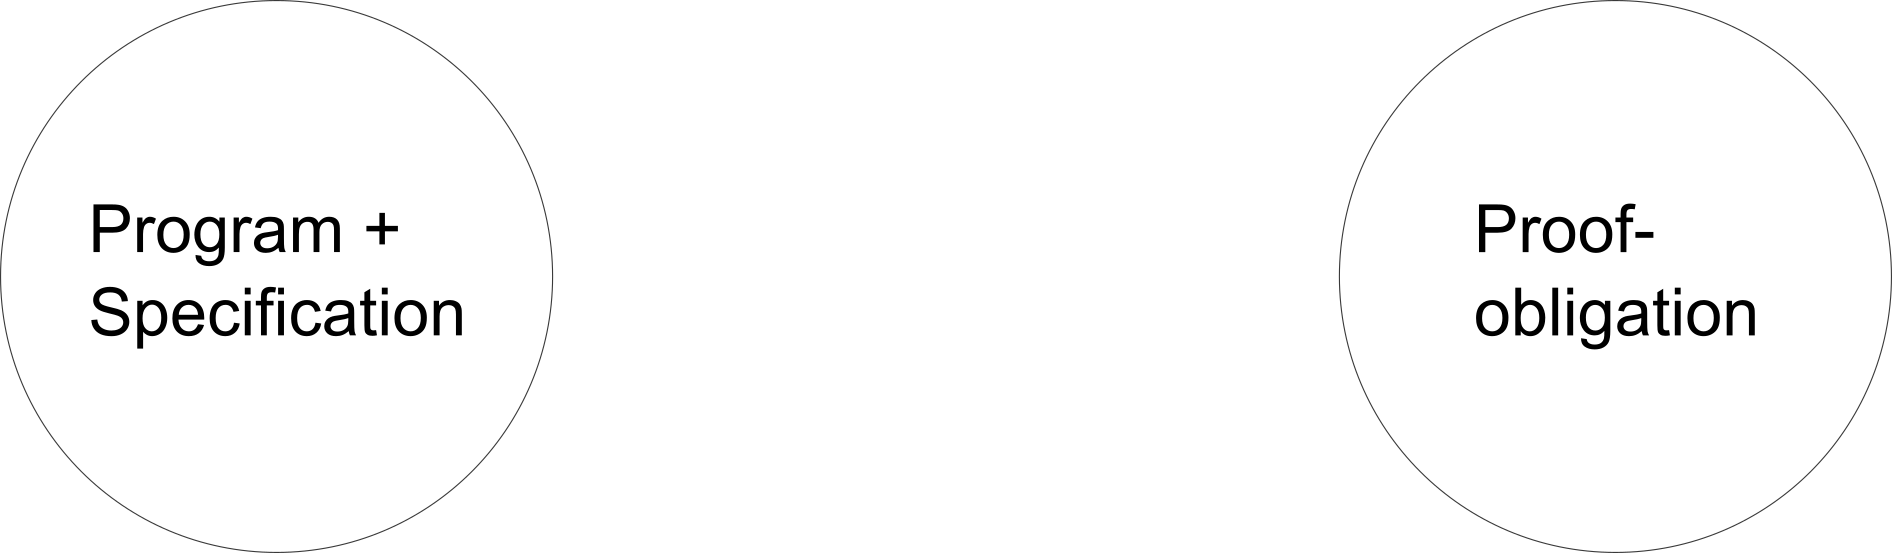
\includegraphics[width=\textwidth]{../../Bilder/base.png}
% \end{frame}

\begin{frame}[c]{Auto-active}
 
\includegraphics[width=\textwidth]{../../Bilder/AutoActive.png}
  \end{frame}


\begin{frame}[c]{Point-and-Click}
 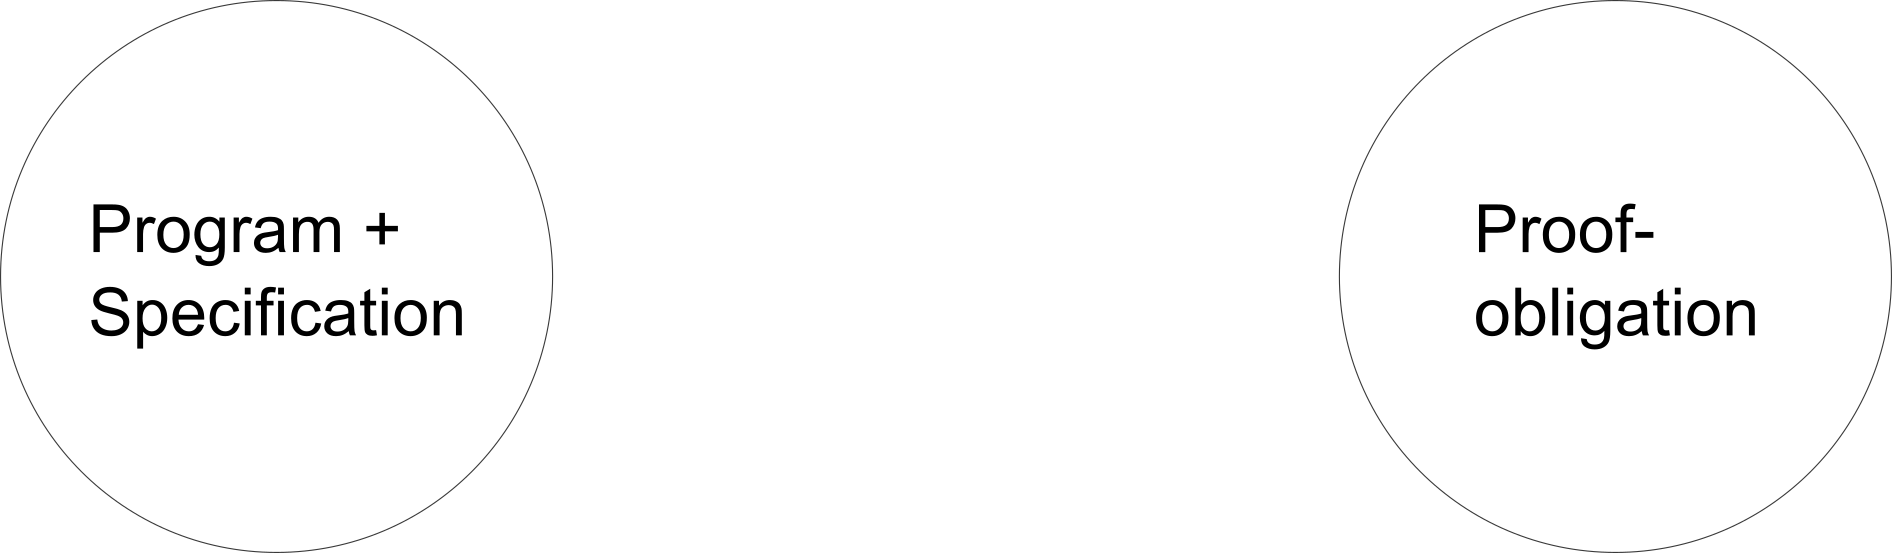
\includegraphics[width=\textwidth]{../../Bilder/base.png}
\end{frame}


\begin{frame}[c]{Point-and-Click}
 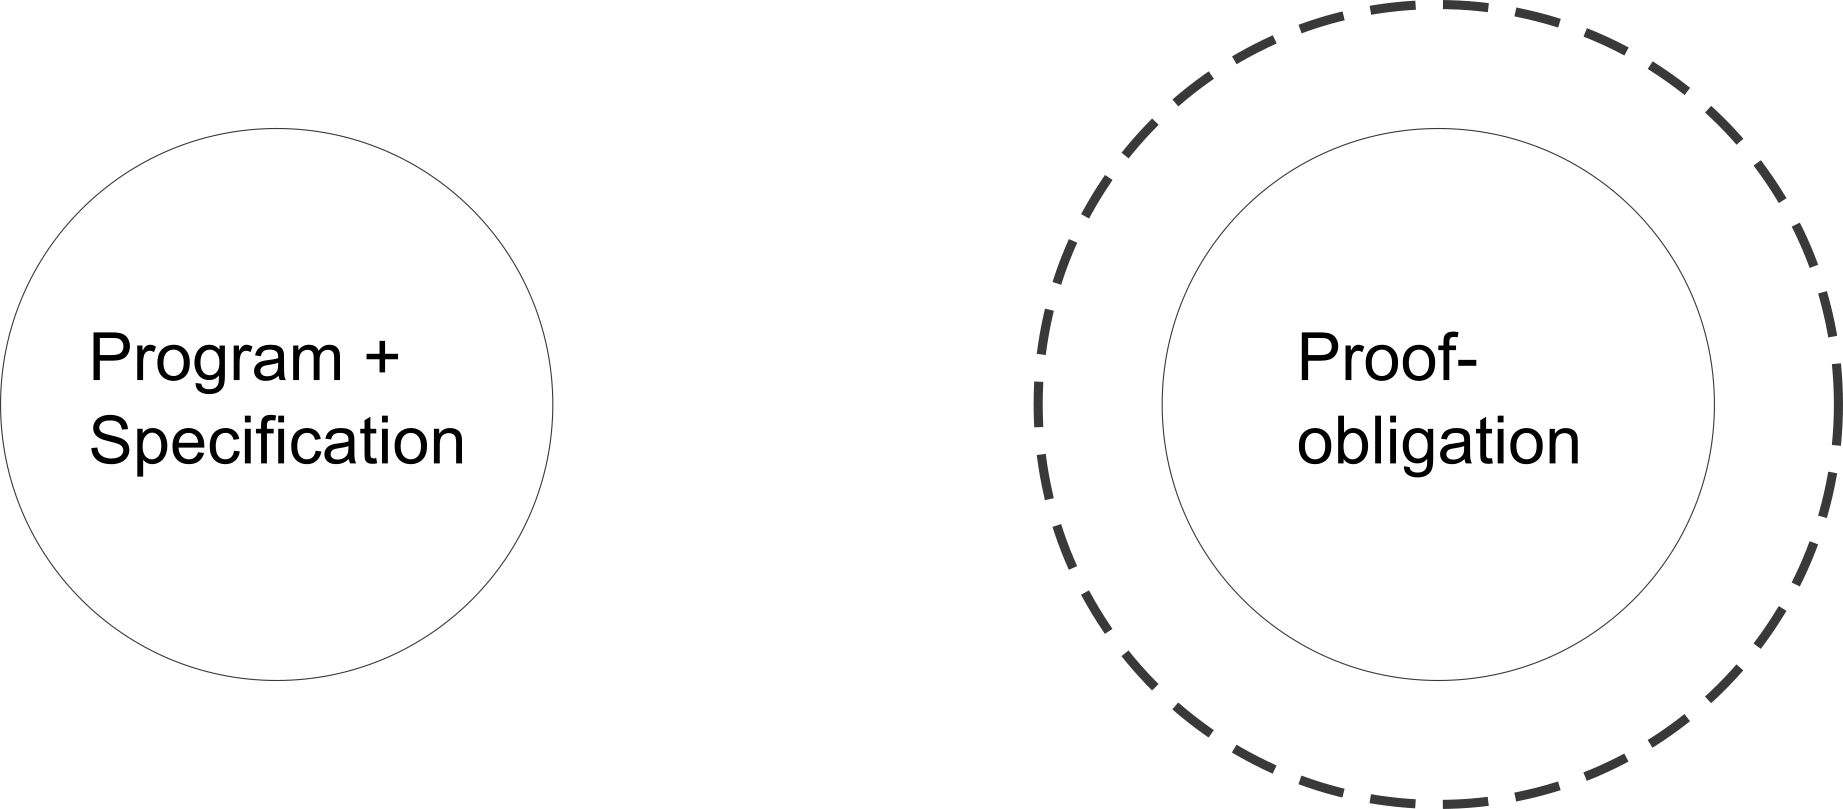
\includegraphics[width=\textwidth]{../../Bilder/PC.png}
\end{frame}


\begin{frame}[c]{Point-and-Click}
 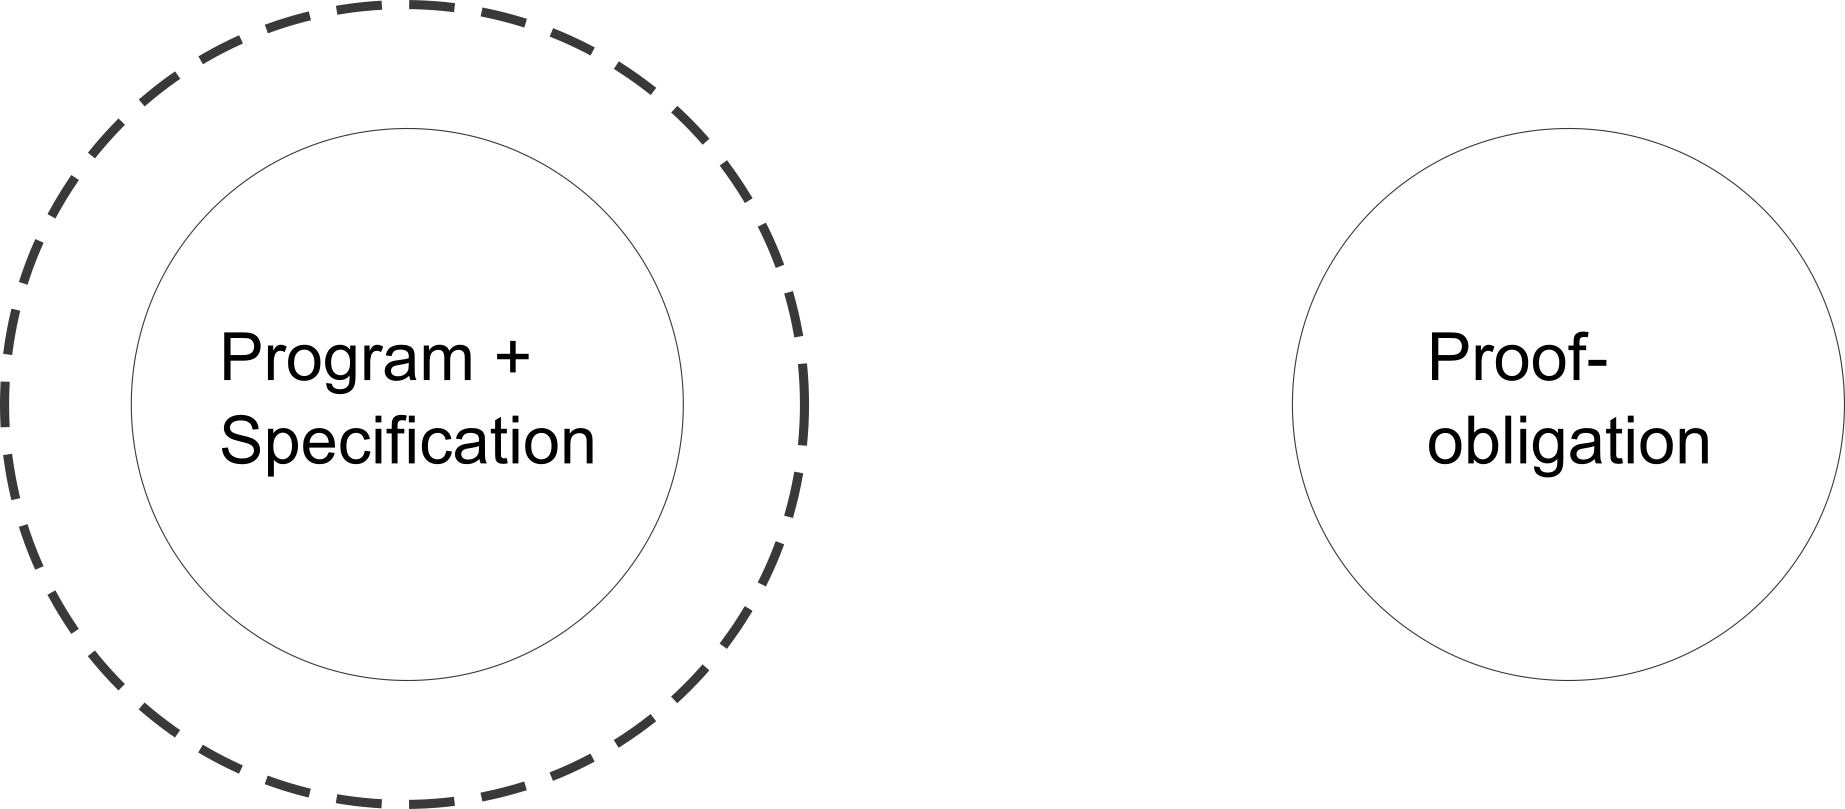
\includegraphics[width=\textwidth]{../../Bilder/PC1.png}
\end{frame}

\begin{frame}[c]{Point-and-Click}
 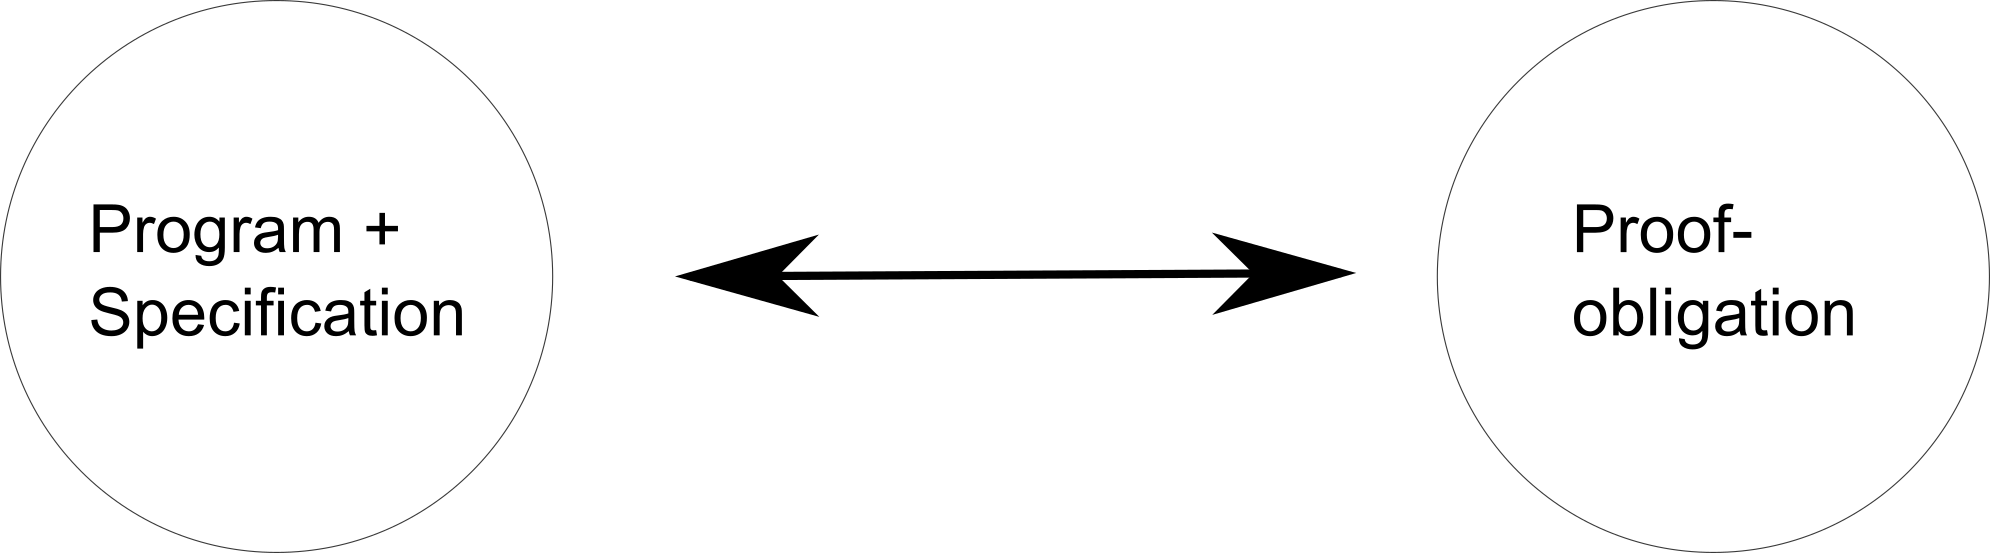
\includegraphics[width=\textwidth]{../../Bilder/PC2.png}
\end{frame}

\begin{frame}[c]{Text-based}
 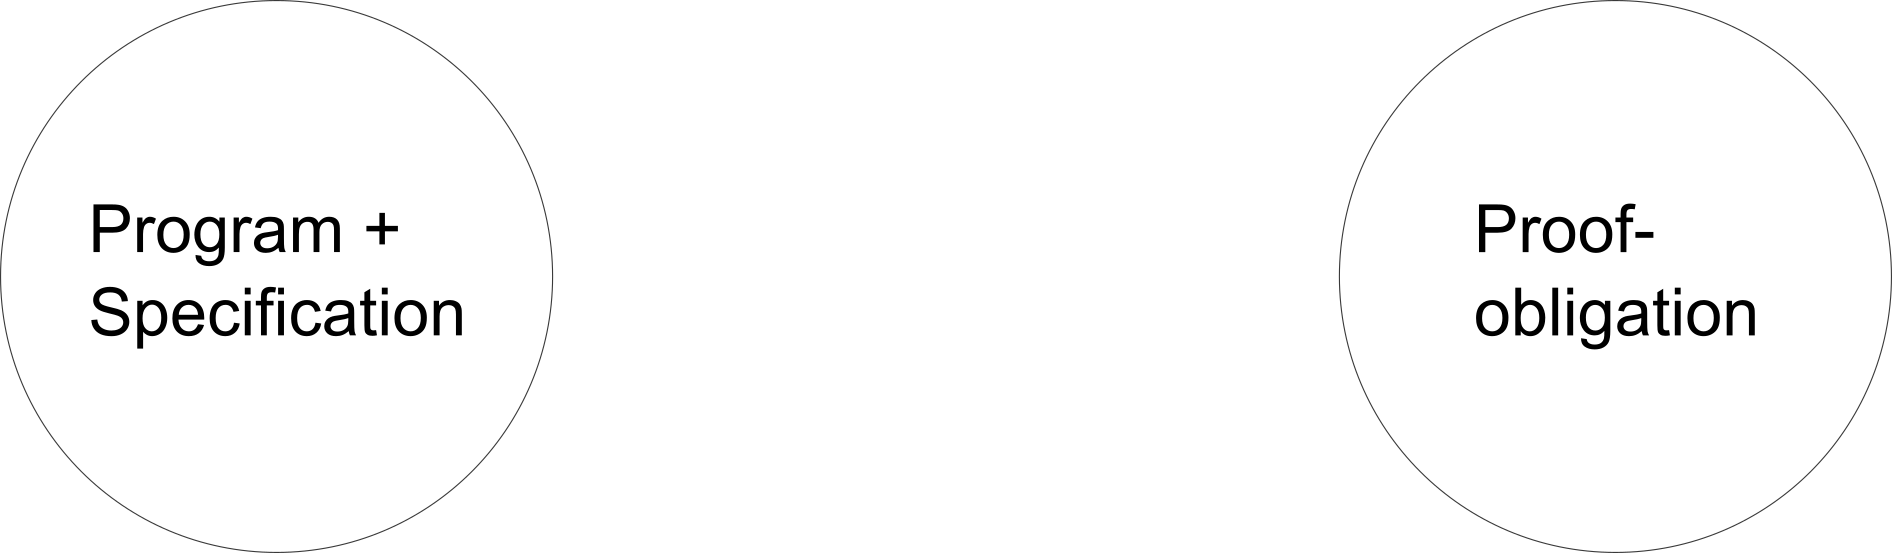
\includegraphics[width=\textwidth]{../../Bilder/base.png}
\end{frame}

\begin{frame}[c]{Text-based}
 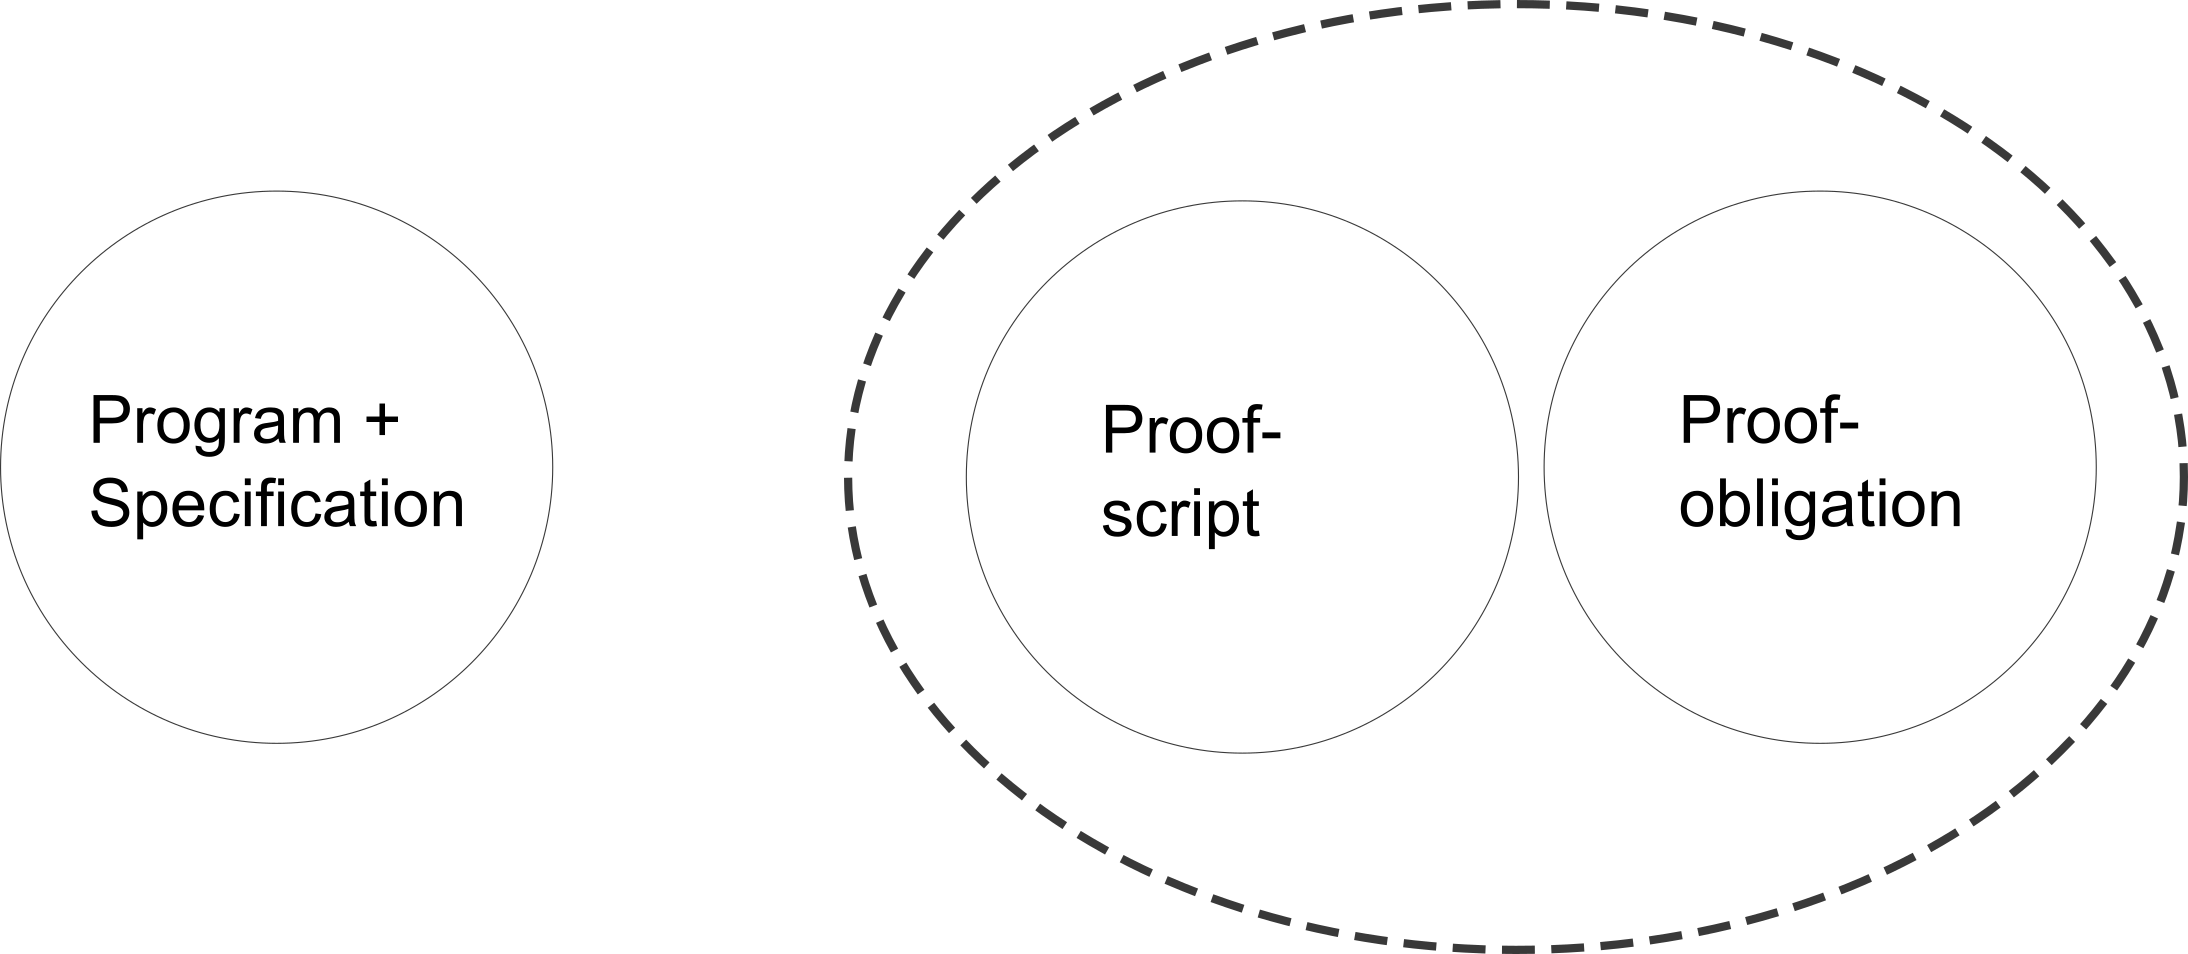
\includegraphics[width=\textwidth]{../../Bilder/script.png}
\end{frame}

\begin{frame}[c]{Problems with Interaction in State-of-the-Art Systems}
 \begin{itemize}
  \item interaction on different views
  \item hidden-dependencies between views
  \item context change for the user cognitively challenging
  \item interaction on different abstraction-levels 
  \item missing interaction possibilities in views
 \end{itemize}

\end{frame}


% 
% Ein Tool, um Interaktionskonzepte umzusetzen und zu erproben, welche
% einen möglichst nahtlosen Übergang zwischen den Sichten ermöglichen und
% gleichzeitig alle Sichten integrieren.
% 

\begin{frame}[c]{Goal of our concept}
 An interactive program verification system that allows to implement and research different interaction concepts:
 \begin{itemize}
  \item integration of all views
  \item integration of all interaction concepts
  \item seamless transition between views 

 \end{itemize}

\end{frame}


% Folie 5:
% "SunBurst Diagramm":
% Hypothese: Nutzerinteraktion benötigt, je nach Kontext, a) einen
% fokussierten Blick auf bestimmte Elemente oder b) einen Überblick über
% einen größeren Zusammenhang.
% 
% => Dafür ist ein Kontextwechsel notwendig
% => dieser erfordert mentale Kapazitäten
% => Ziel ist es dabei die Last für den Nutzer zu reduzieren
% mit a) Anzahl der Elemente zu reduzieren und b) den Aufwand einzelner
% Wechsel zu verringern

\begin{frame}[c]{Hypothesis}
 User interaction needs, depending on the context, 
 \begin{enumerate}[(a)]
  \item a focussed view on specific elements or
  \item an overview of the bigger picture.
 \end{enumerate}

% \begin{block}{Consequence:}
%  A context change is needed, which demands cognitive load from the user.\\
%  \bigskip
%  Goal: Reduce load for user
% \begin{itemize}
%  \item reduce number of elements
%  \item reduce effort for change
% \end{itemize}
% \end{block}

\end{frame}

\begin{frame}[c]{Structure of the Program Verification Problem}
 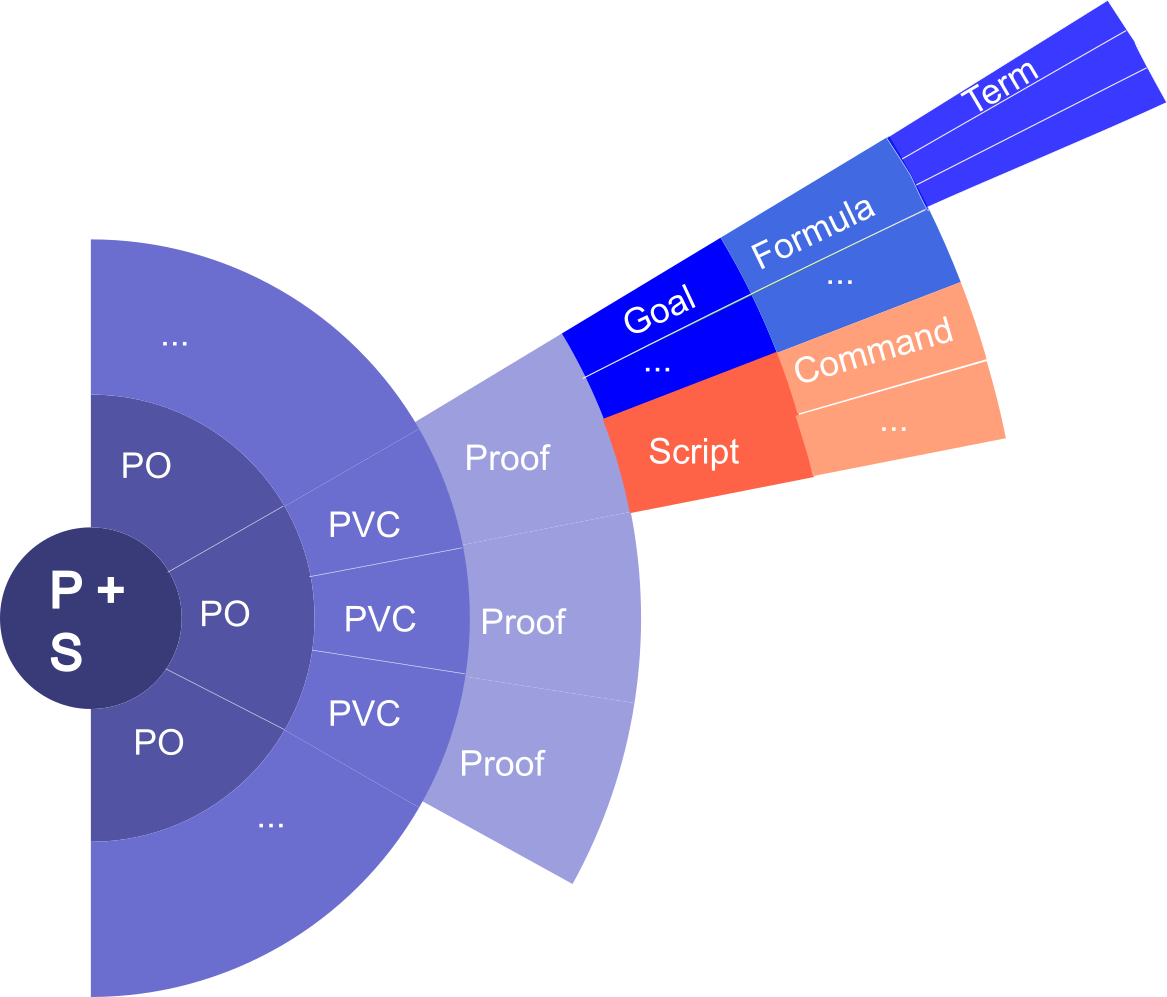
\includegraphics[width=.7\textwidth]{../../Bilder/sunburst1.png}
\end{frame}

\begin{frame}[c]{Objectives}
The user is ...
 \begin{enumerate}
  \item ... able to use appropriate view at all times
  \item ... can easily switch views
  \item ... is able to determine the results of costly actions before executing them  
 \end{enumerate}

\end{frame}

\begin{frame}[fragile]{Objective 1: Appropriate View at All Times}
The user needs different views (problem and user dependent)
\bigskip
 \begin{enumerate}[(a)]
  \item overview over the whole system state (global system state, proof state, remaining proof tasks, ...)
  \item tailor-made views that focus on a specific part of the proof problem (e.g., single proof verification condition)
 %   \item integrate all views into one system 
%   \item show overview over tasks (show system state)
%   \item allow light-weight tools to discharge simple proof obligations (let the user concentrate on hard tasks)
%   \item support overview and focussing onto one proof verification condition 
 \end{enumerate}
 \bigskip
 Our concept integrates all views into one system and allows suitable interaction on the views.
\end{frame}

\begin{frame}[c]{Objective 2: Easy switch of Views}
For the user: Switching view is switching context.\\
$\Rightarrow$ requires cognitive resources\\
\bigskip
Goal: Reduce cognitive resources for context switch by supporting fluent switches between views:\\
\bigskip
\begin{itemize}
\item show similar things in proximity to each other (e.g., adjacent elements of problem structure)
\item show effect of user interaction in all visible views to keep track of changes
\item show dependencies between entities to make hidden dependencies clear
%   \item always show two adjacent views
 \end{itemize}
 
\end{frame}

\begin{frame}[c]{Objective 3: Determine Action Results}
Show the user different variant of the \emph{future} (principle of least surprise).\\
\bigskip
\begin{itemize}
 \item allow light-weight tools to discharge simple proof obligations ($\Rightarrow$ let the user concentrate on hard tasks)
 \item reduce unrecoverable errors by showing action results in context
 \item integration of proof exploration techniques
\end{itemize}

 
\end{frame}

% Folie 6:
% Genauere Ziele:
% * Nutzer kann jederzeit die geeignete Sicht verwenden
% * Es wird dem Nutzer leicht gemacht die Sichten zu wechseln
% * Es kann dem Nutzer die Auswirkungen seiner Aktionen vorab angezeigt
% werden und zwar im Kontext der Sicht
% 
% Folie 6++: Genauere Beschreibung der Ziele; (geplant ist pro Ziel etwa
% eine Folie):
% 
% 1) Interaktionen auf allen Sichten
% * Einfache Tools auf der Überblickssicht (Damit meine ich die
% Möglichkeit, dass der Nutzer am Anfang sagen könnte "Versuch erst einmal
% Z3 und dann mal sehen was noch offen bleibt")
% * Annotationsbasiert im Code
% * Point & click in Logik-Sicht
% * Scriptbasiert auf der Logiksicht
% 
% 2) Sichtenwechsel erleichtern:
% a) durch Anzeige der Sichten nebeneinander (also zuletzt fokussierte und
% dann die nächste Sicht)
% b) Abhängigkeiten sichtbar machen (über Sichten hinweg)
% 
% 3) Überblick und Fokussierung:
% * Hierarchische Ansicht der Artefakte (DafnyDecls, PO, PVC, ...)
% * Gruppierung
% * Ansicht der Ergebnisse der zu beweisenden Aussagen
% 
% 4) Zukunft anzeigen um Fehler zu vermeiden und Zahl der Iterationen zu
% verringern
% * Anzeigen der Änderungen im Kontext
% * Erlauben von Beweis-Explorationsmöglichkeiten
\begin{frame}{Demo}
 
\end{frame}

\end{document}
 
